\chapter{积分}
\label{ch:Integration}

\section*{学习目标}
\begin{todolist}
	\item 理解积分是微分(求导)的逆过程
	\item 积分$(ax+b)^n$
	\item 积分运算的法则,包括函数之和差,固定常数等
	\item 已知某函数的导数,通过积分求算其原函数表达式
	\item 求算定积分的结果
	\item 求算不当积分的结果
	\item 利用定积分求算函数包围的面积,包括两个函数之间包围的面积
	\item 利用定积分求算旋转体的体积
\end{todolist}
\clearpage


\section{积分的意义}
\label{sec:Meaning of Integration}
积分integration是微分differentiation的反向运算,因此有如果$f'(x)$是$f(x)$的导数的话,那么$\int f'(x)\mathrm{d} x=f(x)+C$,即对$f'(x)$求算不定积分,结果必定为含有$f(x)$的一系列函数。
\clearpage


\section{求算积分的运算法则}
\label{sec:Operation rules for integration}
和微分一样,考试中会使用某些函数加加减减进行积分的求算。因此有如下的一些运算法则。在这里不做证明,仅需利用即可

\subsection*{幂次函数的积分}
由于积分和求导之间互为逆运算的关系,因此,如果对幂次函数进行积分的话,其表达式为:
\[
	\int x^n \mathrm{d} x= \frac{1}{n+1} \cdot  x^{n+1} + C
\]

\subsection*{加减法以及固定倍数}
\begin{align*}
	\int kf(x)\mathrm{d} x &= k\cdot \int f(x)\mathrm{d} x\\
	\int f(x)\pm g(x) \mathrm{d} x &=\int f(x) \mathrm{d} x+ \int g(x) \mathrm{d} x
\end{align*}

\begin{ExampleBox}
Evaluate $\int (2x^3-5x+1) \mathrm{d} x$
\tcblower
分解为三个部分分别进行积分即可。\\
\begin{align*}
\int (2x^3-5x+1) \mathrm{d} x &= \int 2x^3 \mathrm{d} x -\int 5x \mathrm{d} x+\int 1 \mathrm{d} x\\
					&= 2\int x^3\mathrm{d} x -5 \int x\mathrm{d} x +x\\
					&=2\cdot \frac{1}{4}x^4-5\cdot\frac{1}{2}x^2+x+C\\
					&=\frac{1}{2}x^4-\frac{5}{2}x^2+x+C
\end{align*}

\end{ExampleBox}

\subsection*{求算$(ax+b)^n$的积分}
利用\gls{substitution}可以求算$\int (ax+b)^n \mathrm{d} x$这样的积分,结果为
\[\frac{1}{a\cdot (n+1)}\cdot (ax+b)^{n+1}+C\]

\begin{SummBox}
推导过程如下:
首先令$u=ax+b$,可知$\frac{\mathrm{d} u}{\mathrm{d} x}=a$,等价于$\mathrm{d} u= a\cdot \mathrm{d} x$\\
因此该定积分可以改写为:
\[
	\int (ax+b)^n \mathrm{d} x =\int u^n \cdot \frac{1}{a} \mathrm{d} u
\]
利用之前所讲的积分法则得到:
\[
	\frac{1}{a} \cdot \frac{1}{n+1}\cdot u^{n+1}+C
\]
将$u$替换回$ax+b$即可
\end{SummBox}

\subsection*{根据导数求算原函数}
A-Level考试中经常需要解决如下的问题:
\begin{ExampleBox}
A curve is such that $\frac{\mathrm{d} y}{\mathrm{d} x}=3x^2 + ax + b$. The curve has stationary points at $(-1, 2)$ and $(3, k)$. Findthe values of the constants $a$, $b$ and $k$.\\
\mbox{}\hfill Adapted from $2019$ spring paper13.
\tcblower
第一步,已知当$x=-1$和$x=3$时,原函数为stationary point。因此其\emph{导数}必定为$0$
\begin{align*}
 3\cdot(-1)^2+a\cdot (-1) +b &=0 \\
 3\cdot3^2+a\cdot3+b &=0
\end{align*}
联立方程得到$a=-6$,$b=-9$。因此\emph{导数}的具体表达式为$\frac{\mathrm{d} y}{\mathrm{d} x}=3x^2 -6x -9$\\

第二步,已知导数,可以通过积分进行\emph{原}函数的求算
\[
	\int 3x^2 -6x -9 \mathrm{d} x =x^3-3x^2-9x+C
\]

第三步,已知$(-1,2)$是在原函数图像当中的点,带入到\emph{原}函数表达式中,可以确定常数$C$的值:
\[
	2= (-1)^3-3\times (-1)^2-9\times(-1)+C
\]
得到$C=-3$,原函数为$y=x^{3}-3x^{2}-9x-3$\\

第四步,将$x=3$带入到函数表达式中,得到纵坐标为$-30$

\begin{figure}[H]
\centering
\includegraphics[width=0.8\textwidth]{s19-qp-13-Q8}
\caption{驻点为$(-1,2)$和$(3,-30)$的原函数图像}
\end{figure}
\end{ExampleBox}
\clearpage


\section{定积分}
\label{sec:Definite Integral}
之前讨论的内容是\gls{iinte}。学会求算不定积分之后,就能够求算\gls{dinte}。

\subsection*{定积分的求算}
首先会在不定积分的基础上增加上下限,其次计算结果为一个常数值。和\gls{iinte}的关系是:
\begin{equation}
\int_{a}^{b}f'(x)\mathrm{d} x=f(b)-f(a)
\tag{Fundamental Law of Calculus}
\label{eq:FTC}
\end{equation}
其中\ref{eq:FTC}也被称之为牛顿莱布尼兹公式。是微积分的基本定理。强调了微分与积分的之间互为逆运算的关系。


\subsection*{广义积分/反常积分}
当中在积分上下限中包含无穷,或者间断点,通常是$\int_{a}^{\infty}f'(x)\mathrm{d} x$或者是$\int_{0}^{b} f'(x)\mathrm{d} x$的类型,对于这类无法直接带入上下限,或者函数无定义的情况,采用极限的手段来求算这一类积分。一般会改写为
\[
	\lim_{b\to \infty} \int_{a}^{b} f'(x) \mathrm{d} x \qquad \lim_{a\to 0} \int_{a}^{b} f'(x) \mathrm{d} x
\]
利用极限的形式进行求算。
\begin{ExampleBox}
Evaluate$\int_{0}^{1}x^{-\frac{1}{2}} \mathrm{d} x$
\tcblower
首先明确这是一个反常积分,因为将下限值$x=0$带入到被积函数中是无意义的。

然后先求算不定积分 $\int x^{-\frac{1}{2}} \mathrm{d} x$得到\emph{反导函数}$f(x)=\frac{1}{-\frac{1}{2}+1}\cdot x^{\frac{1}{2}}=2\cdot x^{\frac{1}{2}}$\\

接下来改写为极限的形式:
\[
	\lim_{a\to 0} f(1)-f(a) =\lim_{a\to 0} 2-2\cdot \sqrt{a}=2
\]
\end{ExampleBox}
\clearpage


\section{定积分的运用}
\label{sec:Application of Definite Integral}
微分是非常实用的,积分也是非常实用的  \makebox{}\hfill adapted from鲁迅

\subsection*{定积分的几何含义}
$\int_{a}^{b} f(x) \mathrm{d} x$这样的表达式本质上代表着函数$y=f(x)$,$x=a$,$x=b$,以及 $x$轴包围起来的图形的面积,如果该面积都在$x$轴上方,则其值为正值;如果在$x$轴下方,结果为负值。(前提是下限$a$要小于上限$b$)

如下图所示:
\begin{figure}[H]
\centering
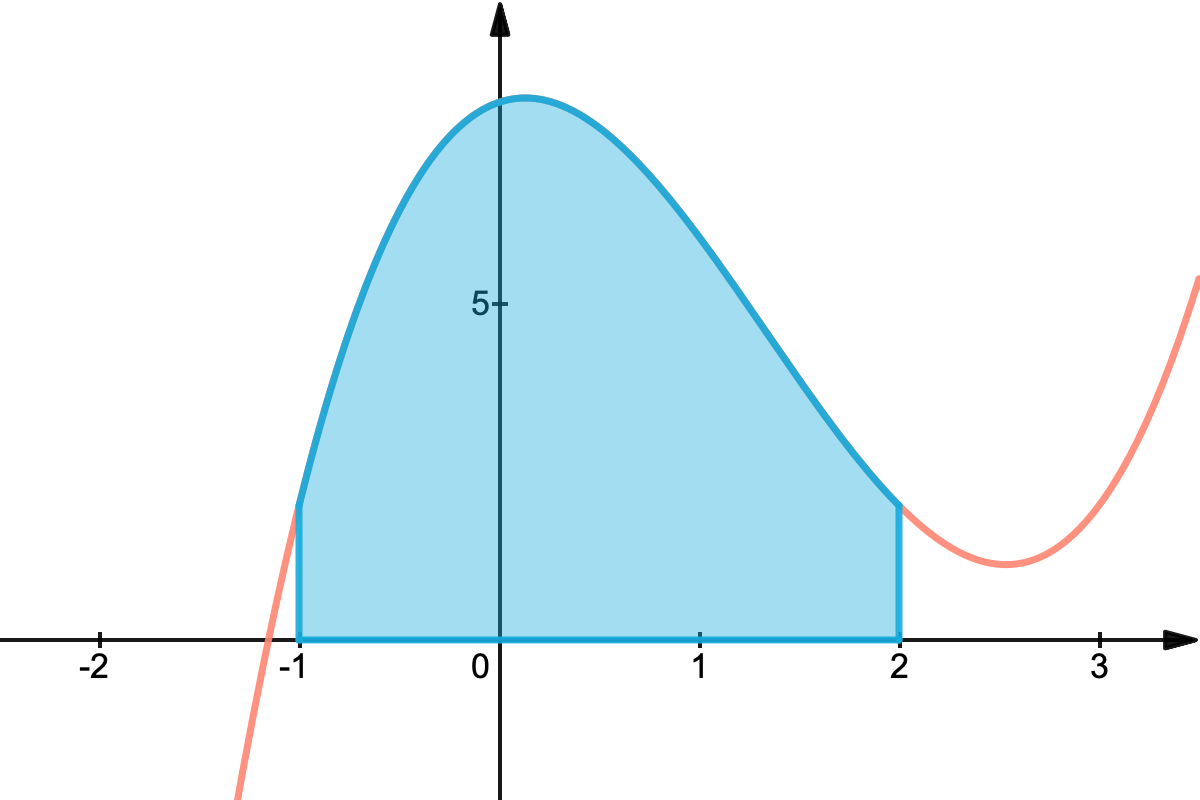
\includegraphics[width=0.8\textwidth]{geometricalmeaning}
\caption{定积分代表函数包围的面积}
\end{figure}




\subsection*{两个函数包围的面积}
求算由两个函数$f(x)$和$g(x)$包围的面积时
\begin{SummBox}
第一步需要找出积分上下限,或者两个函数的交点,$f(x)=g(x)$,确定出$x=a$和$x=b$作为积分上下限;\\
第二步,列出面积积分表达式$A=\int_{a}^{b} f(x)-g(x) \mathrm{d} x$(高的减去低的);\\
第三步求解定积分就可以了
\begin{figure}[H]
\centering
\includegraphics[width=0.8\textwidth]{verticalarea}
\caption{通过竖直方向的无限分割求算面积}
\end{figure}
\end{SummBox}

但是注意,有的情况下需要水平切割,因此微元是$\mathrm{d} y$,那么积分的上下限需要转换为$y$的最大最小值,且要变成$x_2(y)-x_1(y)$。面积就可以用
\[
	\int\limits_{y_{\text{min}}}^{y_{\text{max}}} x_2(y)-x_1(y) \mathrm{d} y
\]
如下图所示
\begin{figure}[H]
\centering
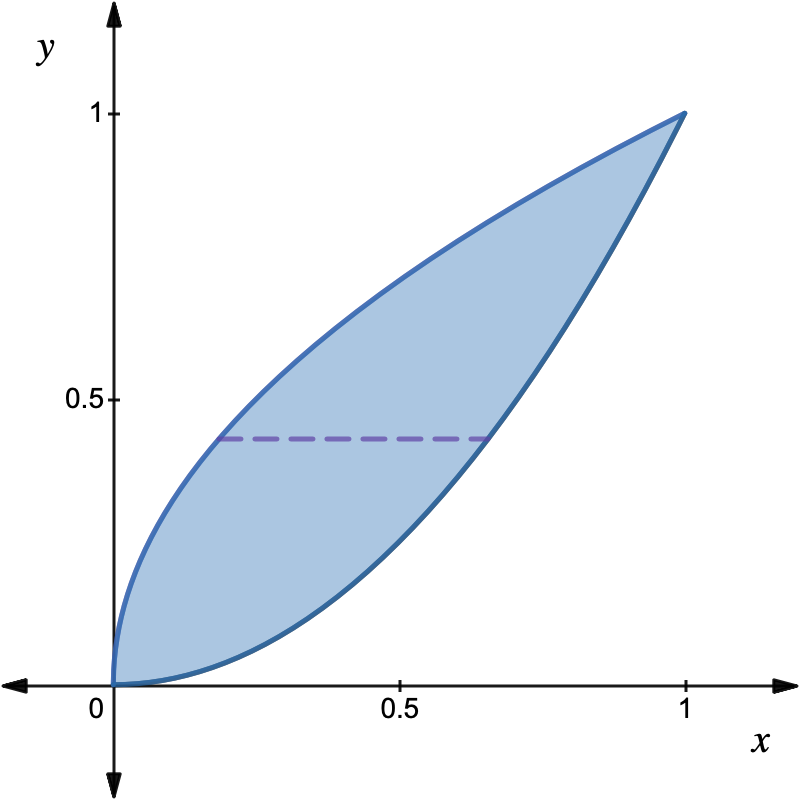
\includegraphics[width=0.8\textwidth]{horizontalarea}
\caption{微元的厚度应该改写为$\mathrm{d} y$}
\label{fig:水平切割}
\end{figure}

\begin{TaskBox}
已知\ref{fig:水平切割}中的两条函数表达式分别为$y=\sqrt x$ 和 $y=x^2$。请将该表达式标注在对应的函数图像范围内,并且标记两个函数的交点,尝试求算这两个函数包围的面积。
\end{TaskBox}

\subsection*{旋转体的体积}
求算某一个函数绕$x$轴旋转所形成的旋转体的体积,需要明白微元绕$x$轴转出来的结果是一个薄薄的disc或者washer。这个薄圆片的厚度是$\mathrm{d} x$,表面积为$\pi r^2$。所以只需要找出来半径$r$与$x$的表达式即可。因此最后求算定积分即可$\int_{a}^{b}\pi (f(x))^2 \mathrm{d} x$。
\begin{figure}[H]
\centering
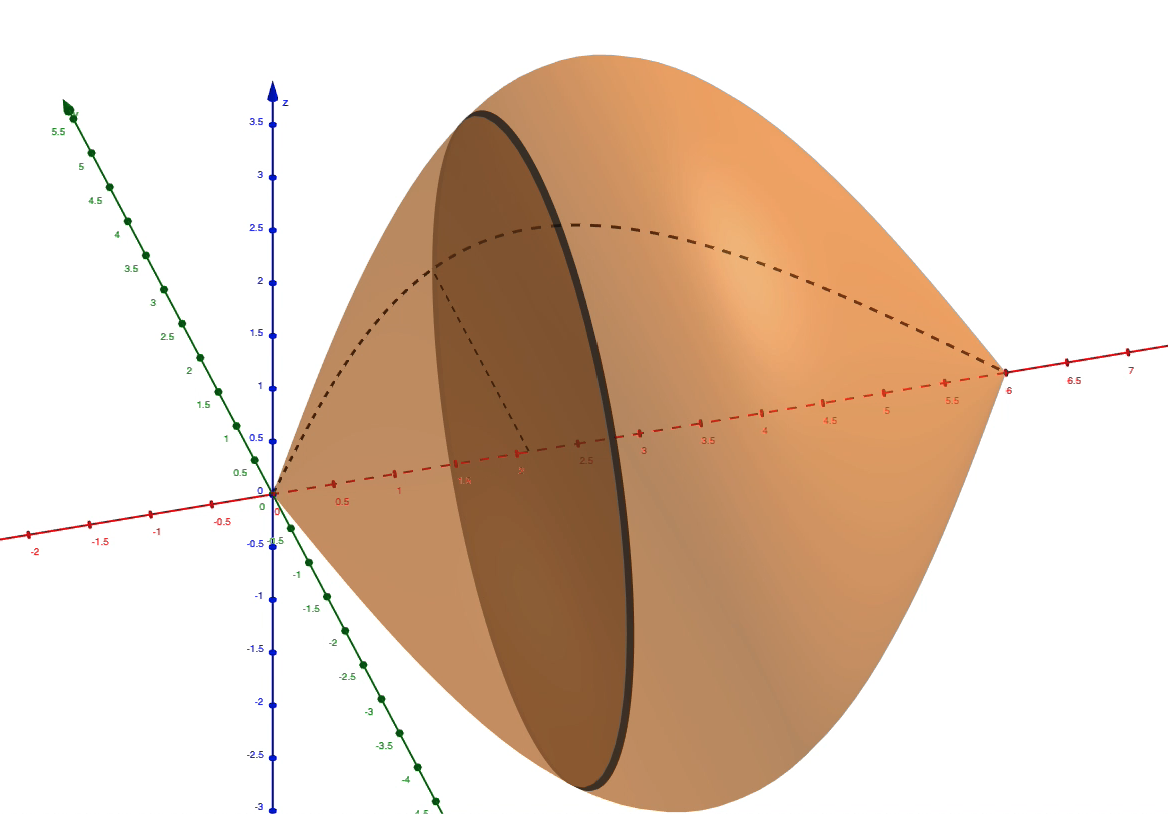
\includegraphics[width=0.8\textwidth]{diskmethod}
\caption{Disk Method的微元体积都是薄片}
\end{figure}

\subsection*{复杂旋转体的体积求算}
如果是由两个函数包围形成的图形,旋转出来的旋转体是空心的的。因此微元的表面积是两个圆的面积之差,需要改写为$\pi\cdot (r_2^2-r_1^2)$。$r_2$是较大的半径,$r_1$是较小的半径,都是关于$x$的表达式。因此定积分的结果是是$\int_{a}^{b}\pi \left[(f(x))^2-(g(x))^2 \right]\mathrm{d} x$。
\begin{figure}[H]
\centering
\includegraphics[width=0.8\textwidth]{Washer Method}
\caption{WasherMethod的微元是空心的}
\end{figure}
可以点击该\href{https://www.geogebra.org/m/ysmcehhc}{Geogebra}活动动态观察旋转轴,上下限对旋转体体积的影响。

